To complement the preregistered trust analyses, we ran exploratory sentiment analyses on participants' open-response text to quantify whether qualitative valence tracks intervention condition, demographic grouping, and downstream trust change. The goal is to use sentiment as a compact language-derived signal that can reveal heterogeneity in how participants interpret and react to the study materials.

Sentiment was computed per participant as the mean VADER compound score across available response fields (AI Interaction Feeling, Need Model Understanding, Job Screening Feeling, Explanation Comment), with $n=504$ participants.

\textbf{Analysis 1: Overall sentiment distribution and mean differences (Figure~\ref{fig:sentiment1_overview}).} We tested condition and group mean differences with Welch two-sample tests and tested Group $\times$ Condition with an OLS interaction term. Condition (Interactive vs Text): $p = .526$ (non-significant), $d = -0.06$. Group (WEIRD vs Normal): $p = .276$ (non-significant), $d = -0.11$. Group $\times$ Condition interaction: $p = .189$ (non-significant), $\beta = -0.057$.

\textbf{Analysis 2: Trust-change comparisons in one combined low/high sentiment plot (Figure~\ref{fig:sentiment2_trust_change_combined}).} We combined the previous full-sample and population-split trust-change analyses into a single figure with three panels (Full sample, WEIRD, Normal). In the Full sample panel, participants were split using full-sample tercile cutoffs and only the lower/upper terciles were compared ($n_{low}=168$, $n_{high}=168$). In the WEIRD and Normal panels, participants were split evenly into low/high sentiment within each population.

Welch high-vs-low tests in the \textbf{Full sample} were: Overall $p = .537$ (non-significant), Analytical $p = .001$ (significant), Emotional $p = .002$ (significant).

Welch high-vs-low tests in the \textbf{WEIRD subgroup} ($n=120$; $n_{low}=60$, $n_{high}=60$) were: Overall $p = .705$ (non-significant), Analytical $p = .921$ (non-significant), Emotional $p = .623$ (non-significant).

Welch high-vs-low tests in the \textbf{Normal subgroup} ($n=384$; $n_{low}=192$, $n_{high}=192$) were: Overall $p = .334$ (non-significant), Analytical $p = .005$ (significant), Emotional $p = .025$ (significant).

Taken together, sentiment did not differ reliably by condition, group, or their interaction in the full sample (Analysis 1), but high-vs-low sentiment contrasts were associated with analytical and emotional trust-change differences in the full sample and in the Normal subgroup when all trust-change comparisons were visualized in one combined plot.

\begin{center}
\centering
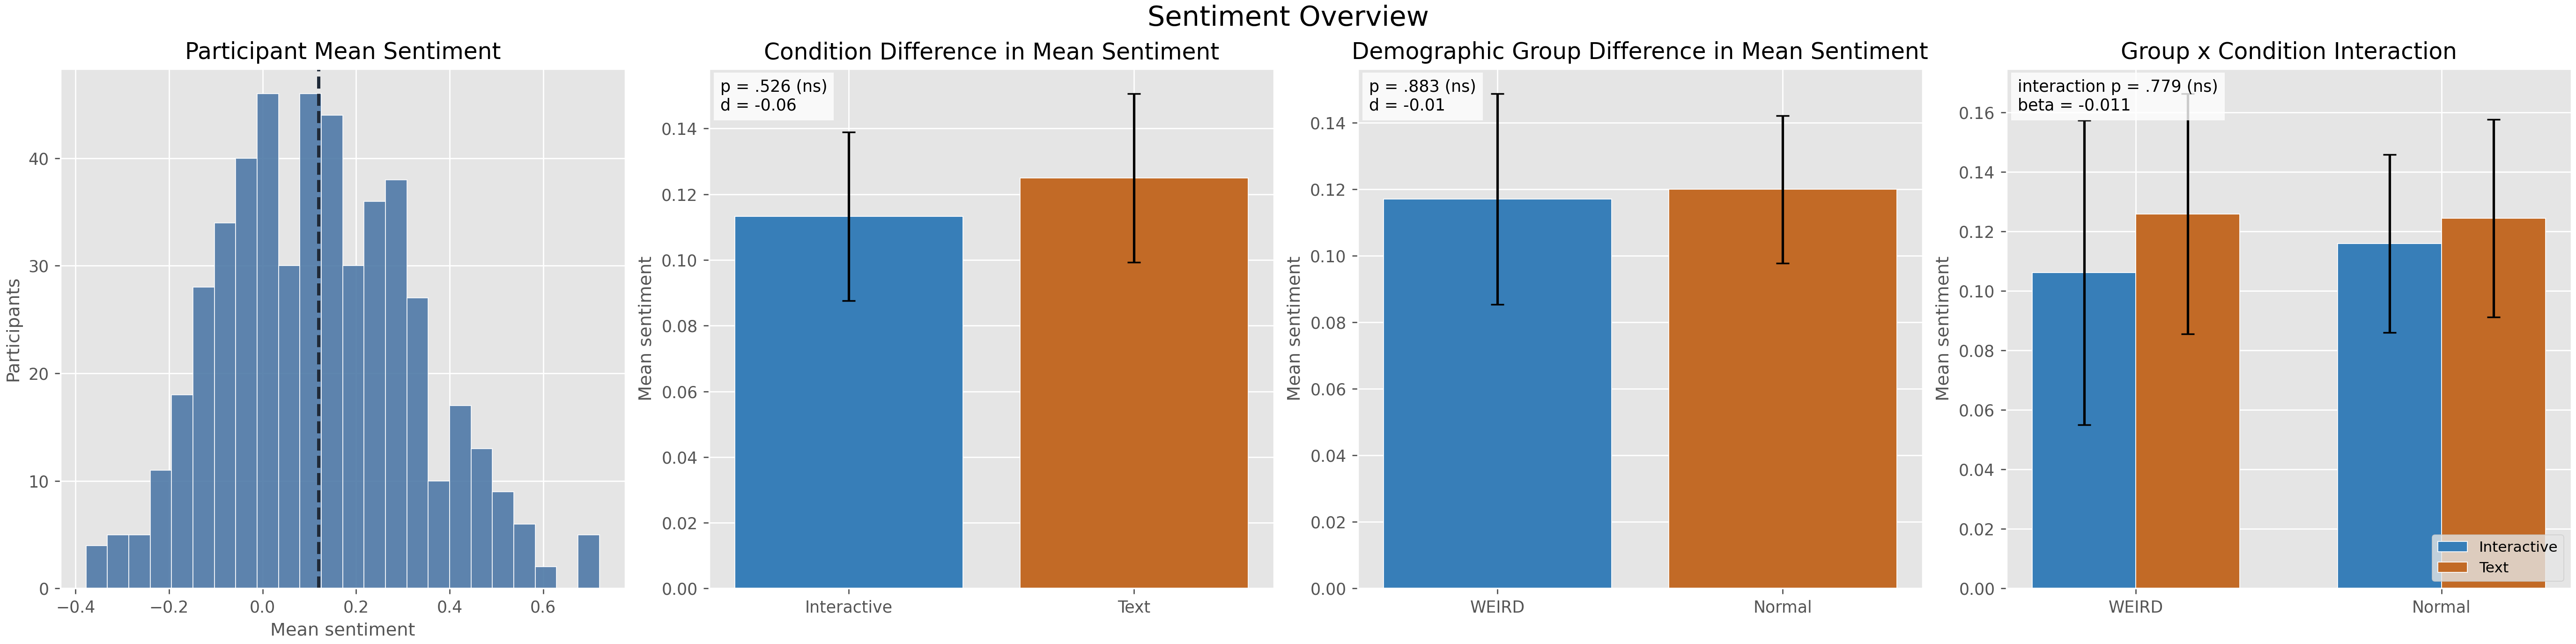
\includegraphics[width=0.98\linewidth]{Figures/sentiment1.png}
\captionof{figure}{Sentiment overview: participant mean sentiment distribution, condition difference, group difference, and Group $\times$ Condition interaction.}
\label{fig:sentiment1_overview}
\end{center}

\begin{center}
\captionof{figure}{Combined high-vs-low sentiment comparison for normalized trust change across the full sample and population splits (WEIRD and Normal).}
\label{fig:sentiment2_trust_change_combined}
\captionof{figure}{High-vs-low sentiment comparison for normalized trust change, split by WEIRD and Normal populations.}
\label{fig:sentiment3_population_split}
\end{center}